\chapter[Fundamentação Teórica]{Fundamentação Teórica}
\label{capFund}

Este capítulo apresenta os principais conceitos que contribui para o entendimento do trabalho. 
Este capítulo está organizado da seguinte forma: Seção \ref{Usabilidade} apresenta o conceito de usabilidade, na seção \ref{Técnicas_de_Avaliação_da_Usabilidade} apresenta as técnicas de avaliação desta usabilidade, na seção \ref{Comunicabilidade} apresentará o conceito de comunicabilidade, na seção \ref{Acessibilidade} apresentará o conceito de acessibilidade, na seção \ref{Experiência_de_Usuário} apresentará o conceito de experiência de usuário \acs{UX}, na seção \ref{Design de Interfaces (UI)} apresentará o conceito de design de interfaces \acs{UI}, na seção \ref{Heurísticas de Jakob Nielsen} será desenvolvido às heurísticas de Jakob Nielsen, na seção \ref{Princípios de Gestalt} será desenvolvido os sete princípios da Gestalt e na seção \ref{Material_Design} apresentará o conceito de \textit{Material Design}.

Para a realização de uma boa avaliação do design e da usabilidade de uma interface e, para conseguir compreender as metodologias que serão abordadas posteriormente, faz-se necessário ter noções básicas sobre alguns conceitos: Usabilidade, \acf{UXD}, Técnicas de Avaliação da Usabilidade, Acessibilidade, Comunicabilidade e \acf{UID}.

\section{Usabilidade}
\label{Usabilidade}
O termo usabilidade tem definições diferentes porque cada autor tem opiniões diferentes. No entanto, há algumas definições que se destacam de outros.

Segundo \citeonline{w3cusabilidade}, a norma ISO9241-11 da \ac{ISO} argumenta que a usabilidade pode ser definida como a eficácia, eficiência e satisfação que os usuários podem atingir por meio de metas específicas para um determinado produto, num determinado contexto (tarefas, equipamentos, ambiente físico e social):

\begin{itemize}
\item \textbf{Eficácia}: avalia se o usuário alcançou os objetivos iniciais da interação, isto é, se conseguiu finalizar a tarefa com sucesso e se obteve bons resultados em termos de qualidade.
\item \textbf{Eficiência}: refere-se à quantidade de esforço e recursos necessários para o usuário alcançar um determinado objetivo. Os desvios e os erros que o usuário realiza durante a interação, auxiliam a avaliar o nível de eficiência da interface.
\item \textbf{Satisfação}: apesar desta ser uma medida subjetiva, refere-se de uma maneira geral ao nível de conforto que o usuário sente ao utilizar a interface e se este se sente satisfeito com os resultados obtidos dado os objetivos iniciais
\end{itemize}

Segundo \citeonline{nielsen-usabilidade}, usabilidade é definida como um atributo de qualidade relacionado à facilidade de o usuário aprender a usar uma determinada interface. Destacando também, 5 fatores de qualidade, que definem a usabilidade:
\begin{itemize}
\item \textbf{Facilidade de aprendizagem}: A interação do usuário com o sistema e a comodidade de realizar tarefas no primeiro contato com a interface;
\item \textbf{Eficiência}: depois de entender o sistema, os usuários devem ser capazes de realizar tarefas de forma rápida e eficiente
\item \textbf{Fácil memorização}: mesmo que não haja interação com a interface após um período de tempo, o usuário deve se lembrar de como ela funciona;
\item \textbf{Erros}: se o usuário cometer um erro, qual é a gravidade desse erro e com que facilidade consegue recuperar do mesmo;
\item \textbf{Satisfação}: a interface deve transmitir confiança e fazer com que os usuários se sintam seguros;
\end{itemize}

A \autoref{Formulários} exemplifica que o \acf{UXD} deve evitar usar apenas cores para indicar erros, colocando uma mensagem apresentando qual foi o erro cometido, também evitar formulários muito longos. Caso isso seja necessário, considerar separar em blocos ou seções lógicas. Assim, o usuário saberá exatamente em qual etapa está, dando uma boa experiência ao usuário na utilização.

\begin{figure}[ht]
	\begin{center}
	    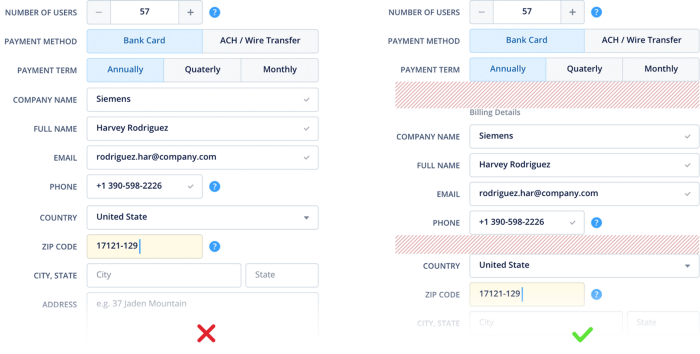
\includegraphics[scale=0.45]{figs/usabilidadeBoaRuim.png}
	\end{center}
	\caption{\label{Formulários}Exemplo de formulários mal elaborados ou confusos.}
    \legend{Fonte: \href{https://i.pinimg.com/564x/5d/66/ce/5d66ce69f103e876c90ab8076c433494.jpg}{https://i.pinimg.com/564x/5d/66/ce/5d66ce69f103e876c90ab8076c433494.jpg}}
\end{figure}

Seja na Web ou em dispositivos móveis, a usabilidade é um conceito importante a se ter em mente ao projetar uma interface, porque se os usuários utilizarem um sistema com baixa usabilidade, não vão querer interagir com ele por muito tempo. Se o aplicativo for complicado de usar, difícil de se obter informações ou se o usuário apenas sentir que está perdido no aplicativo, ele deixará de usá-lo. Claro que existem outros aplicativos para substituí-lo, então o usuário não se preocupará em tentar interagir com sistemas incompreensíveis, e terá medo de cometer erros onde quer que esteja, o que não o deixará confortável e causará estresse e insegurança numa situação que deveria ser simples e intuitiva.

Sendo assim, é considerável que na fase inicial do projeto de qualquer sistema seja feita uma avaliação de usabilidade, não só porque o custo de alterar e melhorar o design é pouco elevado numa fase inicial de desenvolvimento do que após o lançamento no mercado, mas também porque deve-se colocar no mercado uma aplicação útil e com boa usabilidade e que qualquer pessoa consiga facilmente utilizar.

\section{Técnicas de Avaliação da Usabilidade}
\label{Técnicas_de_Avaliação_da_Usabilidade}

Existem vários métodos para estudar e avaliar a usabilidade, porém o mais comum e mais utilizado é o teste com usuários \cite{nielsen-usabilidade}.

Este teste é realizado reunindo um grupo de usuários que possuam ou não conhecimento sobre a aplicação. Este usuários realiza, individualmente, um conjunto de tarefas pré-definidas pela equipe de desenvolvimento da aplicação que, por padrão, correspondem às funcionalidades principais que se quer que a aplicação tenha.

Durante esta etapa, deve-se observar as reações dos usuários durante a interação com a interface e pedir que estes apontem as dificuldades que estão tendo sem nunca interferir no processo, isto é, caso o usuário tenha alguma dúvida sobre como realizar determinada tarefa e questionar sobre isso, somente ao final poderá ser respondida, pois pode-se influenciar e contaminar o resultado do teste, uma vez que já se sabe a resposta e se está testando se o que foi feito é perceptível.

Se para os usuários, realizar essa determinada tarefa não é algo óbvio e intuitivo, então encontrou-se um problema de usabilidade.

Através das dificuldades e problemas apontados pelos usuários, obtém-sesoluções para os mesmos e volta-se a realizar testes com novos usuários para filtrar e encontrar novos os problemas de usabilidade.

\subsection{Avaliação Participativa da Usabilidade}
\label{Avaliação_Participativa_da_Usabilidade}

No âmbito deste estudo, a avaliação participativa desempenha um papel crucial na busca por aprimoramentos significativos na interface do sistema DebugandoED. Diferenciando-se de abordagens tradicionais que dependem exclusivamente de especialistas em usabilidade, nossa metodologia incorpora diretamente as perspectivas dos usuários finais. Este enfoque participativo, centrado na experiência do usuário, visa proporcionar uma avaliação mais alinhada às necessidades reais dos utilizadores.

\section{Comunicabilidade}
\label{Comunicabilidade}
A interface é uma “mensagem” do desenvolvedor/designer para os usuários, com o objetivo de comunicar a quem se destina o sistema, como funciona ou para que serve, quais as vantagens de utilizá-lo e como o usuário deve interagir com o sistema para atingir seus objetivos. Logo, a comunicabilidade destas interfaces são de extrema importância para o usuário entender o funcionamento do sistema \cite{normanDAODESIGNDODIA}

Em sistemas com alta comunicabilidade, os usuários são capazes de responder perguntas como:
\begin{itemize}
    \item Para que o sistema serve?
    \item Qual é a vantagem de utilizá-lo?
    \item Como funciona?
    \item Quais são os princípios gerais de interação com o sistema?
\end{itemize}

O designer deve assegurar que o usuário possa prever e compreender por si só a maneira de utilizar as ferramentas do sistema para realizar as suas atividades com facilidade e eficiência. Caso bem sucedido, o sistema responderá às ações do usuário informando o que está acontecendo, evitando que haja conflitos na interação e, consequentemente, a insatisfação do usuário. Porém, além dessa problemática enfrentada pelo designer, a usabilidade e a comunicabilidade sofrem interferência de outro conceito importante, principalmente em websites, a acessibilidade. 

\section{Acessibilidade}
\label{Acessibilidade}

 \begin{citacao}
 “Acessibilidade é projetar produtos para que pessoas com deficiência possam usá-los. A acessibilidade torna as interfaces de usuário perceptíveis, operáveis e compreensíveis por pessoas com uma ampla gama de habilidades e pessoas em uma ampla gama de circunstâncias, ambientes e condições. Assim, a acessibilidade também beneficia pessoas sem deficiência e organizações que desenvolvem produtos acessíveis” \cite{slhjustask}.
\end{citacao}

A acessibilidade é uma subclasse da usabilidade. Enquanto a usabilidade se preocupa com o universo de todos os potenciais usuários de um sistema, a acessibilidade procura que todas e quaisquer pessoas, independentemente de eventuais limitações sensoriais ou motoras, o possam utilizar. A acessibilidade pretende, com isso, tornar as interfaces perceptíveis e compreensíveis por pessoas em várias circunstâncias, ambientes e condições. A acessibilidade pode ser comparada ao conceito matemático de simetria, segundo o qual algo mantêm as suas características principais depois de submetido a um conjunto de transformações, visto que essas transformações não alteram o objeto ou a sua aparência. \cite{matos2021estudo} 
 
\section{Experiência de Usuário}
\label{Experiência_de_Usuário}

O design experimental é o processo de melhoria da \acf{UX}. Visa tornar o produto útil, localizável e acessível, a interface é fácil de usar, desejável e a informação veiculada é confiável. De acordo com \cite{brito2016usabilidade}, esse processo geralmente é dividido em três etapas:

\begin{enumerate}
    \item \textbf{\ac{UCD}}: fase de pesquisa durante a qual se analisa e se prevê como os usuários utilizarão os produtos. Nesta fase, os seguintes métodos são utilizados para estudar como os usuários percebem, pensam e tomam decisões:
    \begin{itemize}
        \item Análise Competitiva: Pesquisar produtos competitivos e avaliar sua interface e usabilidade. 
        \item Personas: Criar personagens fictícios para ajudar designers a compreender as necessidades dos usuários finais. 
        \item Fluxo de Usuário: diagrama que representa a rota do usuário ao realizar determinadas tarefas. 
    \end{itemize}
   \item \textbf{Usar as informações obtidas na etapa anterior} para executar:
    \begin{itemize}
        \item \textit{Wireframe}: diagrama de baixa fidelidade que representa o layout de um site ou aplicativo. Este permite que se explore e teste ideias de design em projetos iniciais. 
        \item Ensaio: simulação das ações e pensamentos do usuário conforme se avança no \textit{wireframe} passo a passo.
    \end{itemize}
   \item \textbf{Coleta de \textit{feedback} e teste de usabilidade}: Após a fase de \textit{design}, aparece a etapa de coleta de \textit{feedback} da equipe de produto e clientes, também se passa a fazer testes de usabilidade com os usuários, o que auxilia na correção de problemas de usabilidade do aplicativo.
\end{enumerate}

\section{Design de Interfaces}
\label{Design de Interfaces (UI)}
De acordo com \citeonline{maia2016designui}, a \acf{UI} é o recurso que impulsiona a interação humana com produtos físicos ou virtuais. A interface varia de brinquedos e eletrodomésticos a aplicativos móveis ou páginas da web. O trabalho de um designer de interface não se limita a compreender os problemas e necessidades do usuário. Este tipo de projeto envolve conhecimento técnico e estético da construção de ferramentas funcionais. Na prática, o design da interface envolve: partes visuais, usabilidade, arquitetura da informação, navegação e transições de tela. Em outras palavras, todas as funções que aumentam e melhoram a maneira como os usuários lidam com os produtos. Tudo deve ser construído pela satisfação dos fatores humanos. Nesse sentido, a \acf{UX} deve ser o foco de atenção no desenvolvimento de produtos, serviços ou sistemas. Um bom projeto, não importa o quão grande ou pequeno seja, deve passar por um estágio de ideias e necessidades esperadas dos usuários.

A interface bem projetada é principalmente responsável por permitir que os usuários naveguem em sites ou aplicativos. Incentivar e fidelizar esse usuário também é uma meta. Portanto, quando bem pensada, a interface tem a capacidade de se tornar uma ferramenta e facilitar a vida das pessoas. Ignorar a importância do design da interface pode ser o fator decisivo na rejeição de aplicativos. Em suma, o que é importante para os usuários é que o sistema seja fácil de usar e que possa cumprir sua função de criação. Por exemplo, quando alguém usa um aplicativo bancário, deseja que o aplicativo execute a transação principal, evitando assim ir à agência. Portanto, o objetivo do design de interface é ajudar a criar ferramentas atraentes, úteis e eficazes para a solução de problemas \cite{maia2016designui}.

\section{Heurísticas de Jakob Nielsen}
\label{Heurísticas de Jakob Nielsen}

Em 1990, Jakob Nielsen\footnote{em \url{https://www.nngroup.com/people/jakob-nielsen/} está a biografia de Jakob Nielsen e todos os seus trabalhos.} propôs 10 heurísticas que devem ser consideradas ao desenvolver qualquer interface. Nesse caso, as heurísticas referem-se ao senso comum que visa reduzir a sobrecarga cognitiva dos usuários. Portanto, pode tornar a navegação, viagem e experiência melhores, além de reduzir o cansaço. 

Diz-se que as heurísticas de \citeonline{nielsen2005ten} são regras gerais porque não podem determinar diretrizes específicas para usabilidade ou desenvolvimento de interface. Nesse sentido, o método heurístico está relacionado aos anos de experiência e conhecimento do autor.

Com isso, as heurísticas de \citeonline{nielsen2005ten} são:
\begin{enumerate}
    \item \textbf{Visibilidade do status do sistema}: O sistema deve sempre manter os usuários informados sobre o que está acontecendo, por meio de \textit{feedback} apropriado dentro de um período de tempo razoável.
    \item \textbf{Correspondência entre o sistema e o mundo real}: A interface deve ser funcional e acessível que fale a linguagem dos usuários, usando palavras, frases e conceitos familiares ao usuário, em vez de termos técnicos.
    \item \textbf{Liberdade e controle do usuário}: Os usuários geralmente agem por engano, eles precisam de uma ''saída de emergência'' claramente marcada para que ações desnecessárias possam ser deixadas, sem a realização de procedimentos complicados.
    \item \textbf{Consistência e padrões}: Os usuários não devem se perguntar se palavras, situações ou ações diferentes significam a mesma coisa. Siga as práticas da plataforma e do setor. 
    \item \textbf{Prevenção de erros}: Boas mensagens de erro são importantes, porém o melhor design evitará problemas. Elimine condições sujeitas a erros ou conduza inspeções e forneça aos usuários opções de confirmação antes de submeter à operação.
    \item \textbf{Reconhecer ao invés de lembrar}: Minimize a carga de memória do usuário, o usuário não precisa se lembrar de informações de uma parte da interface para outra. As informações necessárias para usar a interface (por exemplo, rótulos de campo ou itens de menu) devem ser visíveis ou facilmente recuperadas quando necessário.
    \item \textbf{Flexibilidade e Eficiência}: Atalhos que não são bem conhecidos por novatos podem acelerar a interação de usuários experientes, de modo que a interface possa servir tanto a usuários inexperientes quanto experientes.
    \item \textbf{Estética e Design minimalista}: A interface não deve conter informações irrelevantes ou raramente necessárias. Cada unidade de informação adicional na interface competirá com a unidade de informação relevante, reduzindo assim sua visibilidade relativa.
    \item \textbf{Auxiliar usuários a reconhecer, diagnosticar e recuperar erros}: A mensagem de erro deve ser expressa em linguagem simples (sem código de erro), apontar o problema com precisão e propor uma solução de forma construtiva. 
    \item \textbf{Ajuda e Documentação}: De preferência, o sistema não requer nenhuma explicação adicional. No entanto, pode ser necessário fornecer documentação para ajudar os usuários a entenderem como realizar suas tarefas.
\end{enumerate}

\section{Gestalt}
\label{Princípios de Gestalt}
O estudo da Gestalt está relacionado à percepção que os usuários vêm do mundo e o que nele contém. Ele explica como o cérebro pode influenciar em determinadas situações, através da interpretação do que se vê \cite{gestalt7principios}.

Ao tentar entender o que nos rodeia, o que a Gestalt sugere é que não se concentre em cada componente pequeno, mas sim em como eles interagem uns com os outros, em sistemas complexos. O princípio da Gestalt desempenha, por isso, um papel importante no desenvolvimento moderno do estudo da sensação e da percepção humana, no design e na publicidade \cite{gestaltleticiasimoes}.

\subsection{Princípios da Gestalt}

Para melhor se trabalhar a Gestalt, seus princípios foram separados em 7:

\begin{enumerate}
    \item \textbf{Princípio da Proximidade:}
    
    Objetos que estão próximos uns aos outros são percebidos, segundo o princípio da proximidade, como mais relacionados do que objetos mais separados. A proximidade diz que quando elementos são posicionados um perto do outro eles são vistos como parte de um grupo, e não individualmente. Eles não precisam sequer ser parecidos, o mero fato de dividirem o mesmo espaço é o suficiente para a proximidade funcionar.
    
    \begin{itemize}
        \item Aplicação na Design \ac{UI}
        
        Assim, algumas das diversas aplicações deste princípio dentro de \ac{UI} se encontram na forma que elementos diferentes são posicionados de forma próxima para formar um grupo.
        
        Na \autoref{proximidade}, os labels estão próximos aos campos para que sejam percebidos como uma coisa só:
        
        \begin{figure}[htb]
        	\begin{center}
        	    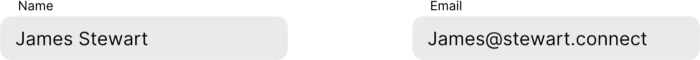
\includegraphics[scale=0.45]{figs/proximidade.png}
        	\end{center}
        	\caption{\label{proximidade}Exemplo de Proximidade}
            \legend{Fonte: \href{https://miro.medium.com/v2/resize:fit:720/0*db8wjIe_ZFTqD4uS}{https://miro.medium.com/v2/resize:fit:720/0*db8wjIe\_ZFTqD4uS}}
        \end{figure}
    \end{itemize}

    \item \textbf{Princípio da Similaridade:}
    
    Usuários percebem objetos que parecem semelhantes como tendo usos semelhantes. Essa é uma estratégia simples que você pode usar em seus designs como meio para comunicar a função de um determinado objeto rapidamente, aumentando a usabilidade.
    
    Ao criar ícones ou estruturas similares, por exemplo, se economiza muito tempo explicando para o usuário qual é a sua função.
    
    \begin{itemize}
        \item Aplicação
        
        Na \autoref{similaridade}, pode-se perceber que os campos têm a mesma função, mas que o botão, apesar de ter forma semelhante, possui outra funcionalidade, já que seu tratamento é diferente.
        
        \begin{figure}[htb]
        	\begin{center}
        	    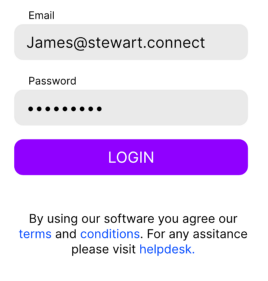
\includegraphics[scale=0.5]{figs/similaridade.png}
        	\end{center}
        	\caption{\label{similaridade}Exemplo de Similaridade}
        	\legend{Fonte: \href{https://miro.medium.com/v2/resize:fit:720/0*yW15A7gQjg6cDsFY}{https://miro.medium.com/v2/resize:fit:720/0*yW15A7gQjg6cDsFY}}
        \end{figure}
    \end{itemize}
    
    \item \textbf{Princípio da Continuidade}
    
    Por mais estranho que isso pareça à primeira vista, o olhar do usuário cria um tipo de impulso à medida que ele se move de objeto para objeto em um layout, e a isso chamamos de continuidade.

    Linhas, em geral, aumentam esse efeito. Tanto que é possível perceber curvas e retas onde elas não existem, apenas pela disposição dos elementos que compõem uma imagem.

    O poder da continuidade se sobrepõe ao poder da cor. Vemos isso aplicado todos os dias nas barras de navegação verticais e horizontais.
    
    \begin{itemize}
        \item Aplicação
        
        Na \autoref{continuidade}, o fato de que o componente de carrossel está cortado nos limites da tela cria esta ilusão e enfatiza a função de se arrastar para ver mais itens.
        
        \begin{figure}[htb]
        	\begin{center}
        	    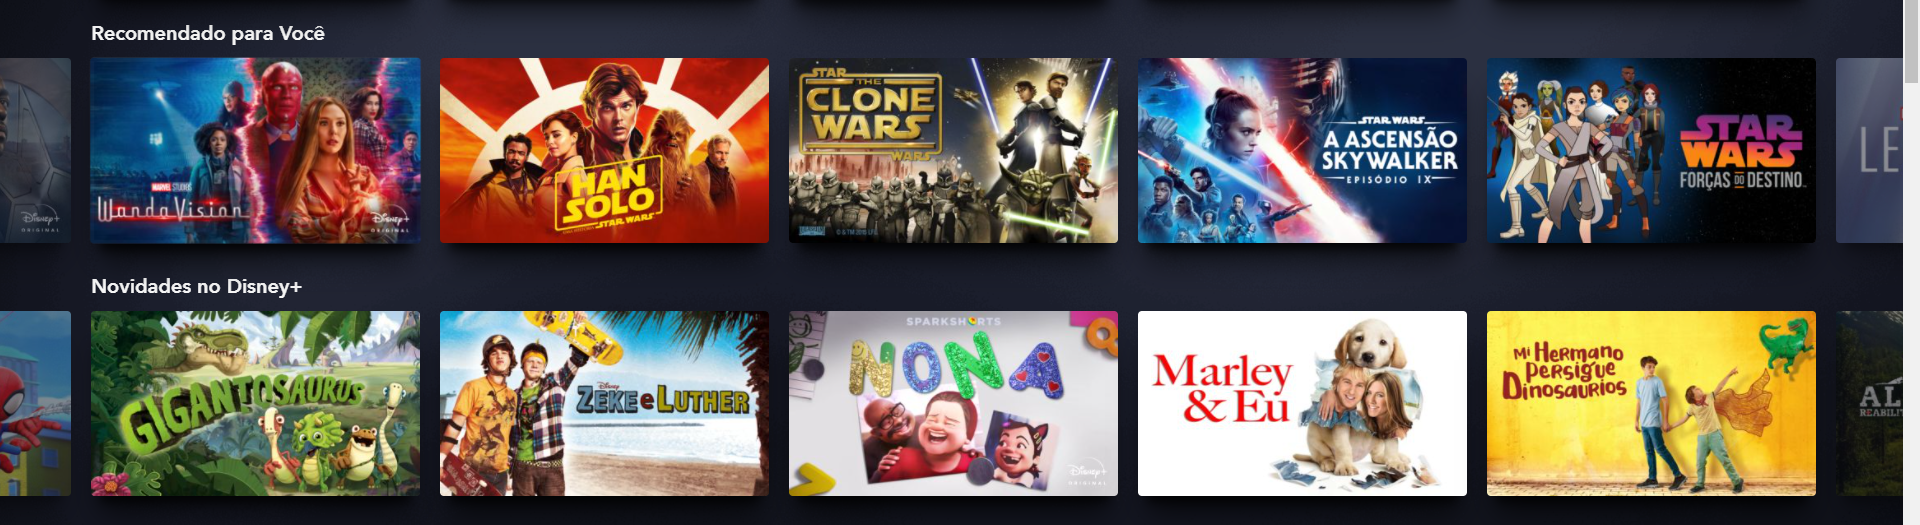
\includegraphics[scale=0.25]{figs/continuidade.png}
        	\end{center}
        	\caption{\label{continuidade}Exemplo de Continuidade}
        	\legend{Fonte: Print da página da Disney Plus \protect\url{https://www.disneyplus.com/}}
        \end{figure}
    \end{itemize}
    
    \item \textbf{Princípio do Fechamento}
    
    O fechamento, por sua vez, aplica as propriedades mencionadas pelo princípio da Gestalt e faz com que usuários completem objetos na sua mente caso eles estejam parcialmente obscurecidos.

    O minimalismo e o uso de elementos parciais emprega o fechamento para economizar espaço e para se comunicar com eficiência.
    
    \begin{itemize}
        \item Aplicação
        
        Na \autoref{fechamento}, a forma com que os elementos são agrupados (utilizando todos os princípios já citados até aqui) cria grupos fechados em si mesmos, mesmo sem que precisemos contornar ou demarcar as seções.
        
        \begin{figure}[htb]
        	\begin{center}
        	    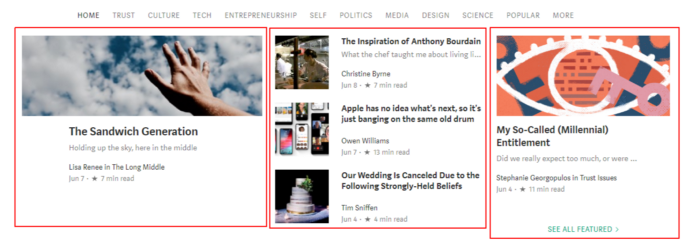
\includegraphics[scale=0.45]{figs/fechamento.png}
        	\end{center}
        	\caption{\label{fechamento}Exemplo de Fechamento}
        	\legend{Fonte: \href{https://miro.medium.com/v2/resize:fit:720/0*43pZlU1PtSsY4AZF}{https://miro.medium.com/v2/resize:fit:720/0*43pZlU1PtSsY4AZF}}
        \end{figure}
    \end{itemize}
    
    \item \textbf{Princípio da Figura-Fundo}
    
    Este princípio afirma que nossa percepção instintivamente percebe objetos como estando à frente ou ao fundo. Pois, como seres humanos, não somos capazes de focar na frente e no fundo simultaneamente, e precisamos escolher apenas um.
    
    \begin{itemize}
        \item Aplicação
        
        Assim, em interfaces, este princípio é amplamente aplicado em navegações, modais e caixas de diálogo. Pode ser observado na \autoref{figura-fundo} que o fundo torna-se secundário quando uma ação que necessita de maior foco é trazida à frente:
        
        \begin{figure}[htb]
        	\begin{center}
        	    \includegraphics[scale=0.45]{figs/figura-fundo.png}
        	\end{center}
        	\caption{\label{figura-fundo}Exemplo de Figura-fundo},
            \legend{Fonte: \href{https://miro.medium.com/v2/resize:fit:720/0*Xb_zAcb44hjXitEa}{https://miro.medium.com/v2/resize:fit:720/0*Xb\_zAcb44hjXitEa}}
        \end{figure}
    \end{itemize}
    
    \item \textbf{Princípio da Região Comum}
    
    O princípio da região comum têm relação com princípio da proximidade, podendo ser até mesmo considerado um sub-princípio deste primeiro. Dessa forma, esse principio afirma que quando objetos são posicionados dentro da mesma região fechada estes são percebidos como parte do mesmo grupo.
    
    \begin{itemize}
        \item Aplicação
        
         Na \autoref{Região Comum} este princípio é amplamente encontrado através da utilização de cards, pois estes criam regiões isoladas de informação, mesmo quando existem diversos cards próximos uns aos outros.
        
        \begin{figure}[htb]
        	\begin{center}
        	    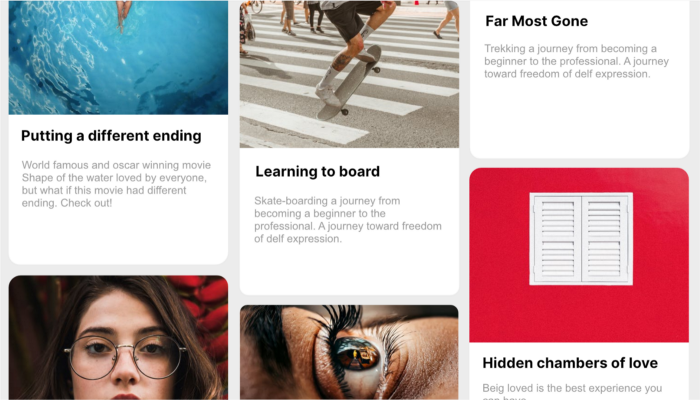
\includegraphics[scale=0.45]{figs/regiao-comum.png}
        	\end{center}
        	\caption{\label{Região Comum}Exemplo de Região Comum}
            \legend{Fonte: \href{https://miro.medium.com/v2/resize:fit:720/0*6SjBY8cq3i95lf_d}{https://miro.medium.com/v2/resize:fit:720/0*6SjBY8cq3i95lf\_d}}
        \end{figure}
    \end{itemize}
    \newpage
    
    \item \textbf{Princípio do Ponto Focal}
    
    O princípio do ponto focal afirma que qualquer elemento que se destacar visualmente vai capturar e prender a atenção de quem está vendo.
    
    \begin{itemize}
        \item Aplicação
        
         Na \autoref{ponto focal} percebe-se que quando é selecionada a parte do corpo, esta se torna em ponto focal. E ao mesmo tempo, o botão verde deixa claro qual é a próxima ação a ser executada
        
        \begin{figure}[htb]
        	\begin{center}
        	    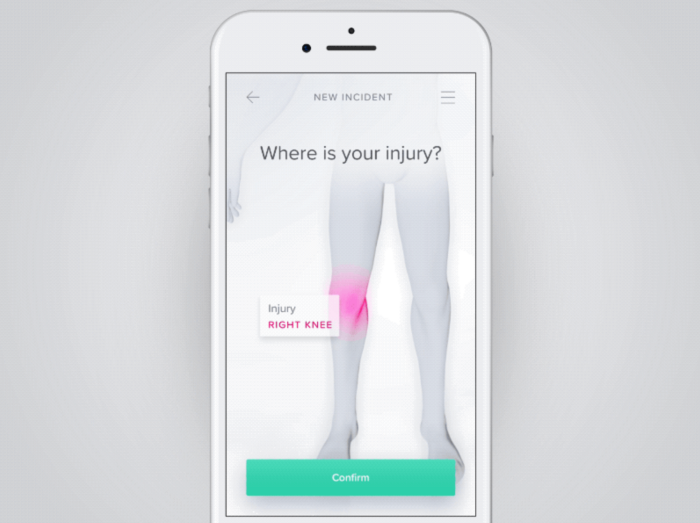
\includegraphics[scale=0.35]{figs/ponto-foca.png}
        	\end{center}
        	\caption{\label{ponto focal}Exemplo de Ponto Focal}
        	\legend{Fonte: \href{https://miro.medium.com/max/700/0*GawJYiOzuiRKBbgq.png}{https://miro.medium.com/max/700/0*GawJYiOzuiRKBbgq.png}}
        \end{figure}
    \end{itemize}
\end{enumerate}


\section{\textit{Material Design}}
\label{Material_Design}
\textit{Material Design} é um conceito visual apresentado pela Google em sua conferência anual que ocorreu em 25 de junho de 2014, a Google I/O\footnote{\url{https://io.google}}.

De acordo com a interpretação de \cite{rodrigues2017aplicaccao}, o \textit{Material Design\footnote{\url{https://material.io/}}} é inspirado em materiais e objetos do mundo real, que reagem de acordo como são manuseados, e vem com várias sugestões para melhorar a experiência da interface do usuário, propondo simplicidade e naturalidade na utilização dos mais diversos tipos de sistemas operacionais.

As principais propostas funcionais deste conceito são os efeitos de animações e transições expressivas, seja de telas inteiras ou objetos, além de efeitos de profundidade, iluminação e sombras realistas, dando a impressão de naturalidade, tornando assim algo virtual tão simples a ponto de fazer o usuário sentir que está fazendo algo extremamente comum e cotidiano sem grande esforço mental.

Para \citeonline{CordeiroFilipeIMD}, a Google tem como intenção desenvolver uma forma única de design que permite ao usuário ter a mesma experiência em todas as plataformas e enumerou 3 conceitos importantes:

\begin{enumerate}
    \item \textbf{O Material é a Metáfora:} O material é baseado na realidade tátil, inspirado no estudo do papel e da tinta, mas tecnologicamente avançado e aberto à imaginação do desenvolvedor. Superfícies e bordas são a prova visual de que tudo é baseado na realidade.
    \item \textbf{Ousado, Gráfico e Intencional:} Os elementos essenciais do design baseado em impressão são: tipografia, grades, espaço, escala, cor e o uso de imagens principais. Esses elementos são mais do que agradáveis aos olhos. Eles criam hierarquia, significado e foco. Opções de cores, aparência de ponta a ponta, tipografia grande e espaço em branco intencional criam uma interface gráfica arrojada.
    \item \textbf{Movimento Fornece Significado:} O movimento respeita e reforça o usuário como motor principal. A ação primária do usuário é o ponto que inicia o movimento. Todas as ações ocorrem dentro de um único ambiente, e os objetos são apresentados ao usuário sem interromper a continuidade da experiência, mesmo quando eles mudam e se reorganizam. O movimento é significativo e apropriado, ajuda a focar e manter a continuidade. O feedback é sutil, mas claro. As transições são eficazes e claras.
\end{enumerate}